\documentclass[12pt]{article}
\usepackage{rotating}
\usepackage[export]{adjustbox}
\usepackage{bm}
\usepackage{empheq}
\usepackage[most]{tcolorbox}
\usepackage{caption}
\usepackage{graphicx}
\usepackage{subfig}
\usepackage{wasysym}
\usepackage[margin=1in]{geometry} 
\usepackage{amsmath,amsthm,amssymb}
\usepackage{hyperref}
\usepackage{algorithm2e}
\usepackage{algorithmic}
\usepackage{float}
\usepackage{multimedia}
\usepackage{tikz} 
\usepackage{atbegshi,picture}
\usepackage{mathtools}
%\usepackage{fourier} 
\usepackage{array}
\usepackage{makecell}
\usepackage{placeins}


\renewcommand\theadalign{bc}
\renewcommand\theadfont{\bfseries}
\renewcommand\theadgape{\Gape[4pt]}
\renewcommand\cellgape{\Gape[4pt]}
\newenvironment{theorem}[2][Theorem]{\begin{trivlist}
		\item[\hskip \labelsep {\bfseries #1}\hskip \labelsep {\bfseries 
			#2.}]}{\end{trivlist}}
\newenvironment{lemma}[2][Lemma]{\begin{trivlist}
		\item[\hskip \labelsep {\bfseries #1}\hskip \labelsep {\bfseries 
			#2.}]}{\end{trivlist}}
\newenvironment{exercise}[2][Exercise]{\begin{trivlist}
		\item[\hskip \labelsep {\bfseries #1}\hskip \labelsep {\bfseries 
			#2.}]}{\end{trivlist}}
\newenvironment{reflection}[2][Reflection]{\begin{trivlist}
		\item[\hskip \labelsep {\bfseries #1}\hskip \labelsep {\bfseries 
			#2.}]}{\end{trivlist}}
\newenvironment{proposition}[2][Proposition]{\begin{trivlist}
		\item[\hskip \labelsep {\bfseries #1}\hskip \labelsep {\bfseries 
			#2.}]}{\end{trivlist}}
\newenvironment{corollary}[2][Corollary]{\begin{trivlist}
		\item[\hskip \labelsep {\bfseries #1}\hskip \labelsep {\bfseries 
			#2.}]}{\end{trivlist}}



%opening
%\title{A high school student friendly way to derive the Jukes-Cantor model }
\title{On the Jukes-Cantor model, distances, and entropy}
\author{Camminady \& Sube}

\begin{document}

\maketitle
\tableofcontents

\begin{abstract}
Lorem Ipsum
\end{abstract}

%\section{Introduction}
%Bio? Teaching? Or leave this out and concentrate on math?
\section{Derivation of the JC69 model via the Poisson distribution}
In the following, we make the same underlying assumptions and simplifications as done in the JC69 model.
\begin{enumerate}
	\item The base frequencies $\pi_A,\pi_C,\pi_G,$ and $\pi_T$ are equal.
	\item The mutation rates are equal and given by $\mu$ being constant in time.
	\item Mutations are point mutations that can happen at any time and are statistically independent.
\end{enumerate}
Furthermore, we assume $X$ to be from the alphabet $\mathcal{A} := \{A,C,G,T\}$ and $s\in \mathcal{A}^n$ is a given DNA sequence of length $n$. However, at first we are going to consider a single base $X$ or alternatively a sequence of length one.
Since the base frequencies are equal we choose $X=A$ to simplify the notation for the following derivation. We are then interested in computing 
\begin{align}
	p_{A,A}(\mu t) = &\text{"the probability that given an initial observation  of base }A\text{,} 	\label{eq:pAA}\\ 
	&\text{ we observe base } A\text{ after an expected number of mutations }\mu t\text{."}
	\nonumber
\end{align}
In theory, there can be an arbitrarily large number of point mutations. Assuming that there are $k$ mutations happening, we are interested in the number of possible mutation sequences that are ending on the same base as they started. For $k=0,1,2$ all possible mutation sequences are illustrated below in Table \ref{table:possible}.
\begin{table}
	\centering
\begin{tabular}{|c|c|c|c|}
	\hline 
	$k$ & Sequences & $n(k)$ & $r(k)$ \\ 
	\hline 
	0& $A$ & 1 & 1 \\ 
	\hline 
	1& $A\rightarrow C$, $A\rightarrow G$, $A\rightarrow T$ & 3 & 0 \\ 
	\hline 
	2& \makecell{$A\rightarrow C \rightarrow A$, $A\rightarrow C \rightarrow G$, $A\rightarrow C\rightarrow T$ ,  \\
	$A\rightarrow G \rightarrow A$, $A\rightarrow G \rightarrow C$, $A\rightarrow G\rightarrow T$, \\
	$A\rightarrow T \rightarrow A$, $A\rightarrow T \rightarrow C$, $A\rightarrow T\rightarrow G$}& 9 & 3 \\ 
	\hline 
\end{tabular}
\caption{Possible mutation sequences for $k=0,1,2$ together with their number $n(k)$ and the number of relevant mutation sequences $r(k)$ ending on $A$.}
\label{table:possible} 
\end{table}
Here, $n(k)$ is the number of possible mutation sequences for a given $k$ and $r(k)$ is the number of those mutation sequences ending on $A$. With $n(k) = 3^k$ it remains to derive an expression for $r(k)$. To do so, consider the step $k-1$. All the sequences that were not relevant, i.e. did not end on $A$, can end on $A$ at step $k$. Thus $r(k) = n(k-1)-r(k-1)$. Together with $n(0)=r(0)=1$ this recursion relation can be solved\footnote{See Appendix for the proof.} to obtain
\begin{align}
	r(k) = \frac14 \left(3(-1)^k+3^k\right),
	\label{eq:rec}
\end{align}
or alternatively 
\begin{align}
q(k) = r(k) / n(k) = \frac{1}{4\cdot 3^k} \left(3(-1)^k+3^k\right),
\label{eq:ratio}
\end{align}
where $q(k)$ is the ratio of mutation sequences of length $k$, ending on $A$.

We now consider the Poisson distribution which allows us to describe the probability of observing a specific number of events, given events that happen statistically independent from another. The only additional information is the expected number of events $\mu t$. Here, $t$ is the time that is considered and $\mu$ the event rate. We can then write
\begin{align}
p_{\text{Poisson}}(\mu t,k) = &\text{" the probability to observe }k\text{ events}\nonumber\\
&\text{ given an expected number of events }\mu t\text{."} \nonumber \\
&= e^{-\mu t}\frac{(\mu t)^k}{k!} \label{eq:poisson}.
\end{align}
Expression \eqref{eq:ratio} and \eqref{eq:poisson} can now be used to compute expression $\eqref{eq:pAA}$. Writing $p_{A,A}$ out in words yields
\begin{align}
	p_{A,A}(\mu t) = \sum_{k=0}^\infty &\text{ "probability to observe $k$ mutations given an expexted number}\nonumber \\  &\text{  of mutations $\mu t$"} \nonumber
	 \cdot \text{"the ratio of mutation sequences ending on $A$."}
\end{align}
This holds true since all of the possible mutation sequences of length $k$ are equally likely. Therefore, the probability of observing a mutation sequence of length $k$ ending on $A$ is solely determined by the ratio $q(k)$. Further computations\footnote{See Appendix for the full computation.} yield the final result
\begin{align}
	p_{A,A}(\mu t) &= \sum_{k=0}^\infty p_{\text{Poisson}} \cdot  q(k) \nonumber
	\\
	&= \sum_{k=0}^\infty e^{-\mu t}\frac{(\mu t)^k}{k!} \cdot \frac{1}{4\cdot 3^k} \left(3(-1)^k+3^k\right) \nonumber	
	\\
	&= \frac14 + \frac34 e^{-\frac43 \mu t}. \label{eq:paa}
\end{align}
Analogously, we can compute $p_{A,A^c}(\mu t)$, i.e. the probability of not finding $A$. This is then
\begin{align*}
	p_{A,A^c}(\mu t) &= 1 - p_{A,A}(\mu t)  \\
	 &= \frac34 -\frac34 e^{-\frac43 \mu t} \\
	 &= p_{A,C}(\mu t) + p_{A,G}(\mu t) + p_{A,T}(\mu t).
\end{align*}
Or equivalently, 
\begin{align}
p_{A,C}(\mu t) = p_{A,G}(\mu t) = p_{A,T}(\mu t) = \frac14 -\frac14 e^{-\frac43 \mu t}.
\end{align}
This exactly matches the probability in the Jukes-Cantor model. Since the base $A$ was chosen without loss of generality, the remaining transition probabilities are to be computed similarly.
\section{Results for DNA sequences}
Given the probabilities $p_{A,A}$ and $p_{A,A^c}$ we can further compute quantities of interest for sequences instead of one single base. 
Let $s_0$ be a DNA sequence and $s_1$ be a second sequence that results from $s_0$ from mutation, given an expected number of mutations per base of $\mu t$. For this, we write $s_0\xrightarrow[]{\mu t} s_1$. Furthermore, we use $|s_0 -s_1|$ to quantify the number of miss matches between $s_0$ and $s_1$. I.e. $|s_0-s_1|=k$ implying miss matches at $k\leq n$ positions.

We can now compute the probability of $s_0$ mutating into \textit{any} $s_1$, observing $|s_0-s_1|=k$. When we observe miss matches at $k$ positions, the sequences have to be equal at $n-k$ positions. Furthermore, there are $\binom{n}{k}$ ways to arrange the $k$ miss matches. Per position that does not match, there are 3 possible bases to fill this position with. Thus in total
\begin{align}
	p(s_0 \xrightarrow[]{\mu t} \text{ any } s_1 \text{ s.th. } |s_0-s_1|=k) =3^k \binom{n}{k} \, \cdot  \left(1-p_{A,A}\right)^{k}\cdot p_{A,A}^{n-k} \label{eq:s0s1}
\end{align}
Similarly, we can compute the probability of some $s_1$ and $s_2$ having difference $k$, assuming they both resulted from two instances of the same sequence $s_0$ due to mutation. Then $s_1$ and $s_2$ have a matching base if they either both do not see a mutation at that position or if the mutation is of the same type for both, e.g. $A\rightarrow C$, $A\rightarrow G$, or $A\rightarrow T$. Then
\begin{align}
p(s_0 \xrightarrow[]{\mu t} \text{ any } s_1  \wedge s_0 \xrightarrow[]{\mu t} \text{ any } s_2  \text{ s.th. } |s_1-s_2|=k) \nonumber \\
 = 3^k\binom{n}{k} \, \cdot \left(1-p_{A,A}^2 -3p_{A,C}^2\right)^{k}\cdot \left(p_{A,A}^2 +3p_{A,C}^2\right)^{n-k},\label{eq:s1s2}
\end{align}
where we write $3p_{A,C}^2$ since $p_{A,C} = p_{A,G}=p_{A,T}$. Again, the choice of $A$ as the origin base does not alter the result. The processes modeled by Eq. \eqref{eq:s0s1} and \eqref{eq:s1s2} are similar in the sense that the second process can be modeled via the first process when doubling the number of expected mutations or equivalently doubling the time while keeping the mutation rate. Indeed, we can verify\footnote{See Appendix for proof.}
\begin{align}
p(s_0 \xrightarrow[]{\mu t} \text{ any } s_1  \wedge s_0 \xrightarrow[]{\mu t}\text{ any } s_2  \text{ s.th. } |s_1-s_2|=k) \nonumber \\ 
= p(s_0 \xrightarrow[]{2 \mu t} \text{ any } s_1 \text{ s.th. } |s_0-s_1|=k).
\label{eq:s1s2equivelence}
\end{align}
Note that for a \textit{specific choice} of $s_1$, the probability of $s_0 \xrightarrow[]{\mu t} s_1$ with distance $k$ is given by $\left(\frac{1-p_{A,A}}{3}\right)^k \cdot p_{A,A}^{n-k}$.

\section{Distances and entropy}
The state of highest entropy goes along with an equilibrium state. Since the equilibrium state favors an equal number of $A,C,G$ and $T$, the state of highest entropy will favor $3/4n$ miss matches (assuming e.g. $s_0=\left(A,...,A\right)\in\mathcal{A}^n$). Given a sequence $s_0$ and a sequence $s_1$ with $|s_0-s_1| = k$, we can ask for the most likely $\mu t$ such that $s_0 \xrightarrow{\mu t} s_1$, i.e. the maximum likelihood estimator (MLE). Given  $s_0$ and $s_1$ with $|s_0-s_1| = k$ we compute 
\begin{align*}
	p_{s_0,s_1}(\mu t)= \left(\frac{1-p_{A,A}}{3}\right)^k \cdot p_{A,A}^{n-k}.
\end{align*}
Differentiating, setting equal to zero and equating for $\mu t$ yields
\begin{align}
	\mu t_{MLE} = -\frac34 \log \left(1-\frac43 \frac{k}{n}\right),
\end{align}
for which the real and imaginary part are plotted in Fig. \ref{fig:distancemeasure}.

If we define 
\begin{align}
	I(p) = -\frac34 \log p,
\end{align}
with $p=1-\frac43\frac{k}{n}$, then $I$ satisfies the "fundamental properties of information"\footnote{\url{https://en.wikipedia.org/wiki/Entropy_(information_theory)}}:
\begin{enumerate}
	\item $I(p)$ is monotonically decreasing in $p$ (increasing probability decreases information)
	\item $I(p)$ is non-negative 
	\item $I(1)=0$ (events that always occur do not communicate information)
	\item $I(p_1 p_2) = I(p_1)+I(p_2)$ (information due to independent event is additive)
\end{enumerate}
\subsection{MLE \& MAP}
Generally, the MLE is given by
\begin{align}
	\mu t_{MLE} = \text{argmax}_{\mu t} f(x | \mu t), 
\end{align}
whereas the MAP is given by
\begin{align}
		\mu t_{MAP} = \text{argmax}_{\mu t} f(\mu t | x) =\text{argmax}_{\mu t} f(x | \mu t) \cdot g(\mu t).
\end{align}
With $g(\mu t)$ being the density of $\mu t$ is the prior. If $g$ is constant, then MAP$=$MEP.
%A sequence of length $n$ can mutate into any of the $4^n$ sequences with different probability. 

\newpage 

\section{Appendix 1 - Graphics}
\begin{figure}[h!]
	\centering
	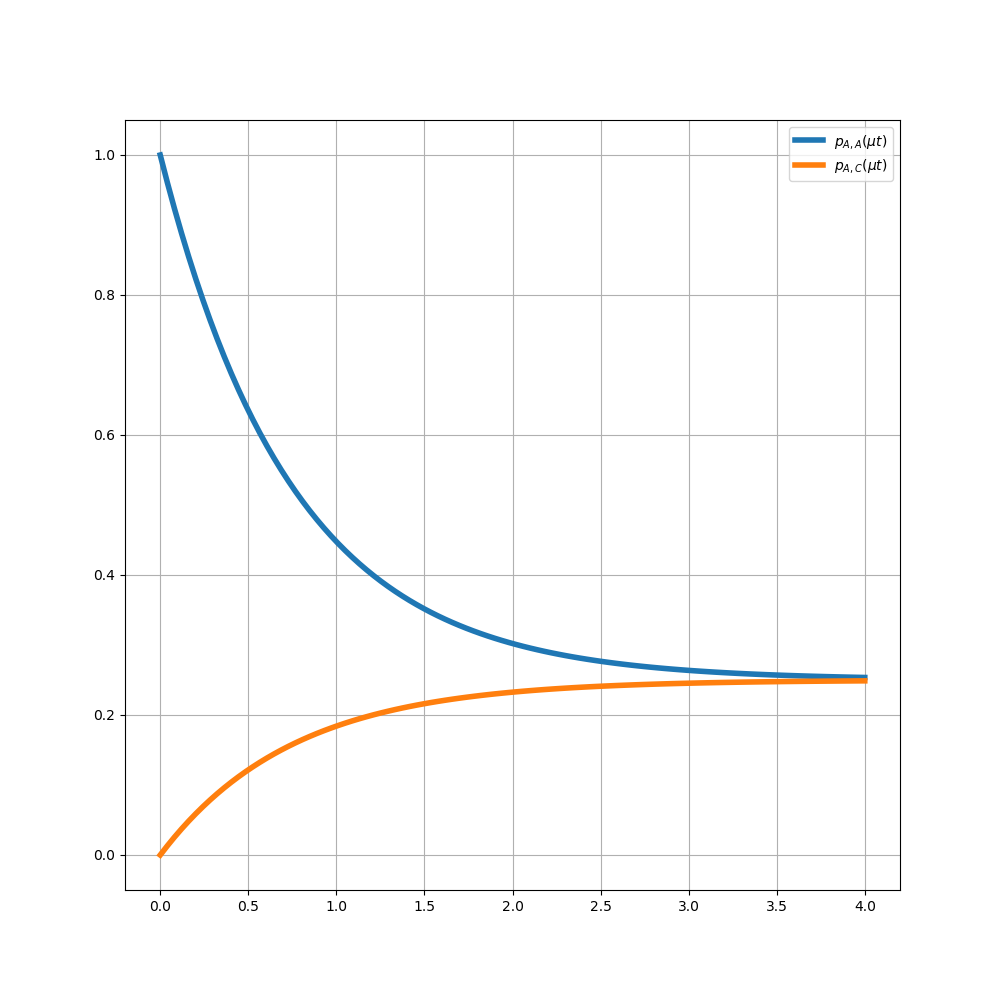
\includegraphics[width=1.0\linewidth]{mutationAAAC}
	\caption{Probability of observing $A$ given $A$ (blue) or observing $C$ given $A$ (orange), depending on $\mu t$.}
	\label{fig:mutationaaac}
\end{figure}
	
\begin{figure}
	\centering
	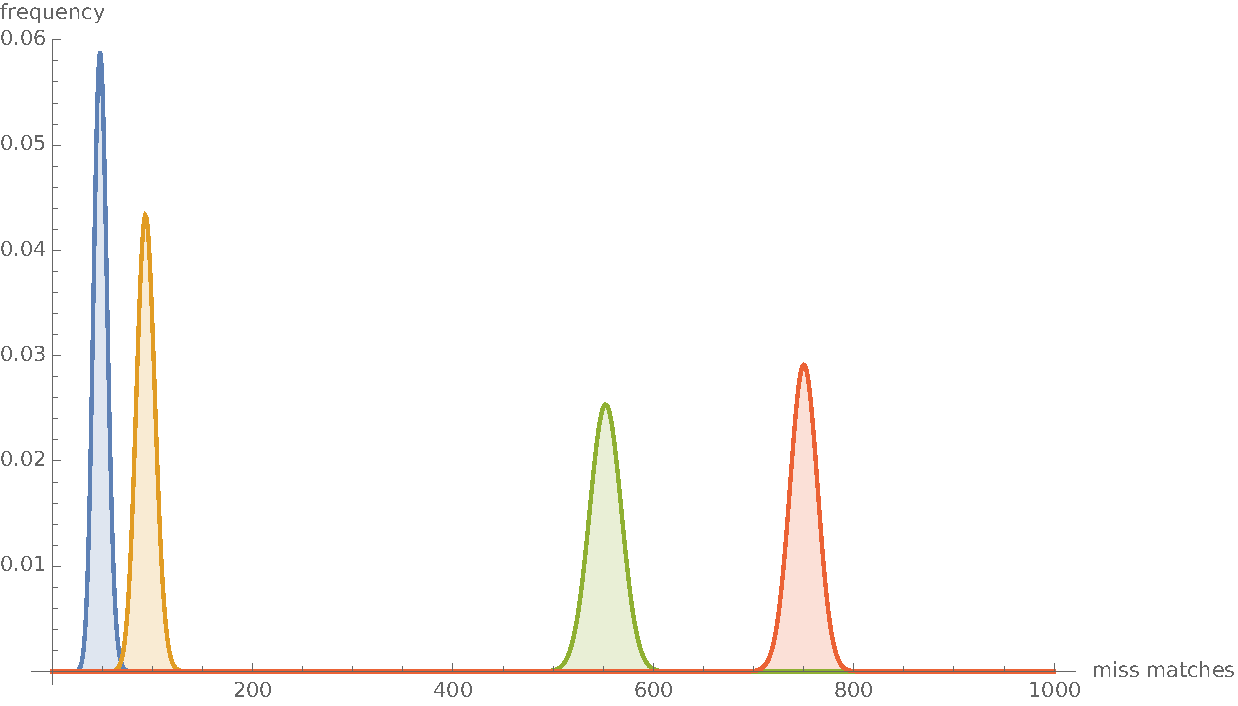
\includegraphics[width=1.0\linewidth]{difference}
	\caption{Given $\mu t$ from small to large, what is the most common difference to a base sequence, considering all mutating sequences w.r.t $s_0$ and $\mu t$. This expression is given by $3^k/4^n \binom{n}{k}\cdot p_{A,A}^{n-k}\cdot p_{A,C}^k$. Plotted for $n=1000$ and $k$ ranging from $0$ to $n$.With $\mu t = 0.05$, $\mu t = 0.1$, $\mu t = 1$ and $\mu t=10$ from left to right.}
	\label{fig:difference}
\end{figure}



\begin{figure}
	\centering
	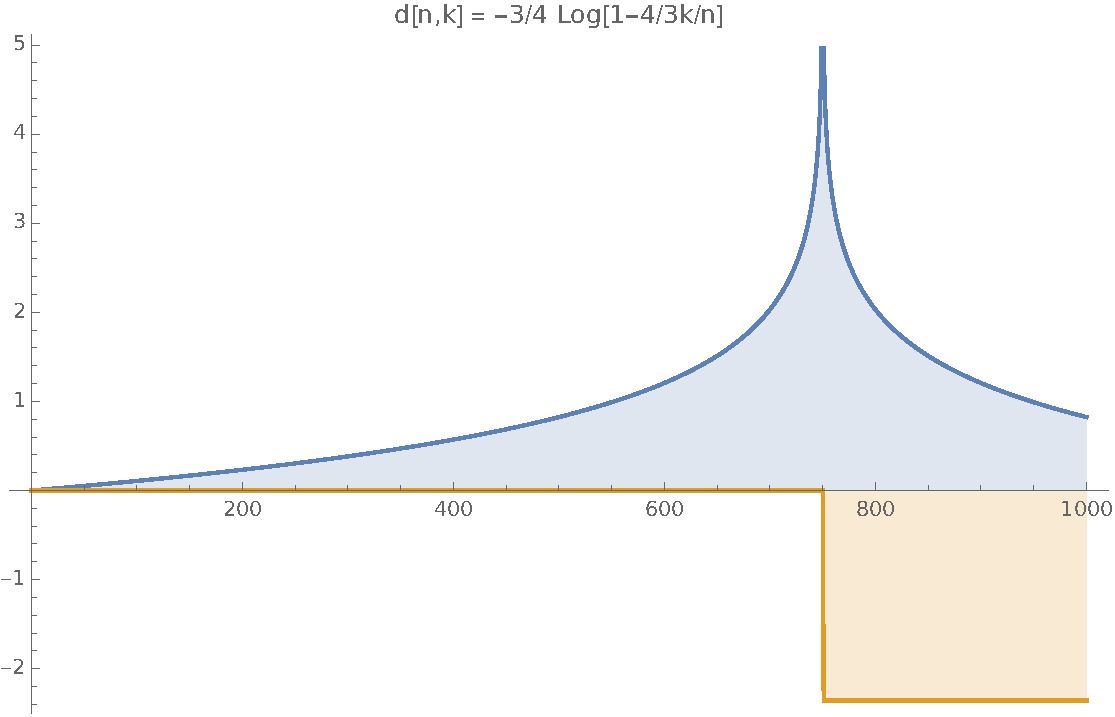
\includegraphics[width=1.0\linewidth]{distancemeasure}
	\caption{Real part (blue) and Imag part (orange). With $g(\mu t,n,k) = p_{A,A}(\mu t)^{n-k} (1-p_{A,A}(\mu t))^k$, we obtain $d$ by differentiating the expression w.r.t $\mu t$ and setting it to zero. I.e. it is the argmax of the expression, meaning the most likely number of expected mutations that yield the observed deviation of two sequences. The expression becomes imaginary for $k\geq 3/4n$ (and diverges for $k=3/4n$). Interestingly, $3/4n$ is also the most likely number of observed miss matches when letting one sequence mutate "for ever". Thus having more than 3/4n miss matches could imply some information loss after which it is no longer reasonable to assume that the two sequences are related? I.e. it there is a higher number of miss matches than what to expect when picking sequences randomly. {\color{red}Note that this is also the exact distance measure as in the JC69 model but with a completely different argumentation.}
	Note2: This can be interpreted as the time we have to wait (given a fixed rate $\mu$) that we have to wait until we observe $k$ miss matches w.r.t original sequence. Since the state of highest entropy is a equal number of bases ($A,C,G,T$), observing more than $3/4n$ miss matches would mean that the entropy would start to decrease again. How is $d$ then related to entropy? }
	\label{fig:distancemeasure}
\end{figure}
\FloatBarrier
\section{Appendix 2 - Proofs}
\begin{proof}[Counting relevant mutation sequences]
	We are going to prove the claim in Eq. \eqref{eq:rec}. 
\end{proof}
\begin{proof}[Computing $p_{A,A}(\mu t)$]
	We are going to prove the claim in Eq. \eqref{eq:paa}.
\end{proof}

\begin{proof}[Equivalence by doubling the timespan]
	We are going to prove the claim in Eq. \eqref{eq:s1s2equivelence}.
	
\end{proof}


\end{document}
